
%%%%%%%%%%%%%%%%%%%%%%%%%%%%%%%%%%%%%%%%%%%%%%%%%%%%%%%%%%%%%%%%%%%%%%%
%% $Id: report.tex,v 1.5 2005/02/09 21:06:42 lindstrm Exp $
%%%%%%%%%%%%%%%%%%%%%%%%%%%%%%%%%%%%%%%%%%%%%%%%%%%%%%%%%%%%%%%%%%%%%%%
%% costhesis usage example
%% modified and added to by GQMJr
%%%%%%%%%%%%%%%%%%%%%%%%%%%%%%%%%%%%%%%%%%%%%%%%%%%%%%%%%%%%%%%%%%%%%%%
%
% The costhesis package accepts the following options
%
%   Document types:
%     msc               - Master Thesis
%     bsc		- Kandidate Thesis
%
%   Layout options:
%
%   Other options:
%     blank             - Removes pagenumbers and headers from empty pages
%     blankmsg          - Prints a message of intent on empty pages
%     scheader          - Typeset headers in SMALL CAPS shape (default)
%     slheader          - Typeset headers in slanted shape 
%
%
%
%

\documentclass[12pt,a4paper,twoside,openright]{book}
%%\documentclass[12pt,a4paper,twoside,openright]{memoir}

\usepackage[msc,blankmsg]{costhesis}
%\usepackage[T1]{fontenc}
%%\usepackage{pslatex}
\renewcommand{\rmdefault}{ptm} 
\usepackage{mathptmx}
\usepackage[scaled=.90]{helvet}
\usepackage{courier}
%
\usepackage{bookmark}


%% ------------------------------------------------------------------
% Equation Packages
%% ------------------------------------------------------------------


\usepackage{times,amsmath,epsfig}
\usepackage[utf8]{inputenc}
\usepackage[usenames,dvipsnames]{color}
\usepackage{amssymb}

\let\labelindent\relax

\usepackage{graphicx}
\usepackage{caption}
\usepackage{hyperref}
\graphicspath{ {images/} }
\usepackage[many]{tcolorbox}
\usepackage{subcaption}
\usepackage{balance}  % for  \balance command ON LAST PAGE  (only there!)
\usepackage{pdfpages}
\usepackage{fancyhdr}
\usepackage{exscale}
\usepackage{booktabs}
\usepackage{multicol}
\usepackage{multirow}
\usepackage{amsfonts}
\usepackage{amssymb}
\usepackage{ntheorem}
\usepackage{paralist}
\usepackage{verbatim}
\usepackage{color}
\usepackage{hyperref}
\usepackage{enumitem}
\usepackage{listings}      % source code
\usepackage{algorithm}
\usepackage{algorithmicx}  % pseudo code (1/2)
\usepackage[noend]{algpseudocode} % pseudo code (2/2)
\usepackage{setspace}
\usepackage{array}
\usepackage{relsize}
\usepackage{diagbox}
\usepackage{listings}


\DeclareMathOperator{\union}{\mathtt{union}}
\providecommand{\myfloor}[1]{\left \lfloor #1 \right \rfloor}

%%%%%%TRIGGER
\algblockdefx[TriggerS]{TriggerS}{EndTriggerS}[2][event]
  {\textbf{trigger} $\langle #1 \rangle$;}

%No extra line - TriggerS 
\makeatletter
\ifthenelse{\equal{\ALG@noend}{t}}%
  {\algtext*{EndTriggerS}}
  {}%
\makeatother

\algblockdefx[Trigger]{Trigger}{EndTrigger}[2][event]
  {\textbf{trigger} $\langle#1$ $\mid$ $#2\rangle$;}

%No extra line - Trigger  
\makeatletter
\ifthenelse{\equal{\ALG@noend}{t}}%
  {\algtext*{EndTrigger}}
  {}%
\makeatother

%%%%%%FOR EACH
\algblockdefx[ForEach]{ForEach}{EndForEach}[2][collection]
   {\textbf{ for each } $#1$ \textbf{as} $#2$}

%No extra line - ForEach
\makeatletter
\ifthenelse{\equal{\ALG@noend}{t}}%
  {\algtext*{EndForEach}}
  {}%
\makeatother

%%%%%%UPON
\algblockdefx[UponEvent]{Upon}{EndUpon}[2][event]
  {\textbf{upon event} $\langle#1$ $\mid$ \emph{#2}$\rangle$ \textbf{do} }

\algblockdefx[UponEventS]{UponS}{EndUponS}[2][event]
  {\textbf{upon event} $\langle#1\rangle$ \textbf{do} }




%%----------------------------------------------------------------------------
%%   pcap2tex stuff
%%----------------------------------------------------------------------------
% \usepackage[dvipsnames*,svgnames]{xcolor} %% For extended colors
% \usepackage{tikz}
 \usetikzlibrary{arrows,decorations.pathmorphing,backgrounds,fit,positioning,calc,shapes}
% \usepackage{pgfmath}	% --math engine
%%----------------------------------------------------------------------------
%\usepackage[latin1]{inputenc}
\usepackage[utf8]{inputenc} % inputenc allows the user to input accented characters directly from the keyboard
\usepackage[swedish,english]{babel}
\usepackage{rotating}		 %% For text rotating
\usepackage{array}			 %% For table wrapping
\usepackage{graphicx}	 %% Support for images
\usepackage{float}			 %% Suppor for more flexible floating box positioning
\usepackage{color}           %% Support for colour 
\usepackage{mdwlist}
\usepackage{setspace}    %% For fine-grained control over line spacing
\usepackage{listings}		%% For source code listing
\usepackage{bytefield}    %% For packet drawings
\usepackage{tabularx}		%% For simple table stretching
\usepackage{multirow}	%% Support for multirow colums in tables
\usepackage{dcolumn}	%% Support for decimal point alignment in tables
\usepackage{url}	%% Support for breaking URLs
\usepackage[perpage,para,symbol]{footmisc} %% use symbols to ``number'' footnotes and reset which symbol is used first on each page

%%\usepackage{pygmentize}  %% required to use minted -- see python-pygments - Pygments is a Syntax Highlighting Package written in Python
%\usepackage[outputdir=.texpadtmp]{minted}
\usepackage{minted}		%% For source code highlighting
\usemintedstyle{borland}


\usepackage{hyperref}		
\usepackage[all]{hypcap}	 %% Prevents an issue related to hyperref and caption linking
%% setup hyperref to use the darkblue color on links
\hypersetup{colorlinks,breaklinks,
            linkcolor=darkblue,urlcolor=darkblue,
            anchorcolor=darkblue,citecolor=darkblue}


%% Some definitions of used colors
\definecolor{darkblue}{rgb}{0.0,0.0,0.3} %% define a color called darkblue
\definecolor{darkred}{rgb}{0.4,0.0,0.0}
\definecolor{red}{rgb}{0.7,0.0,0.0}
\definecolor{lightgrey}{rgb}{0.8,0.8,0.8} 
\definecolor{grey}{rgb}{0.6,0.6,0.6}
\definecolor{darkgrey}{rgb}{0.4,0.4,0.4}
%% Reduce hyphenation as much as possible
\hyphenpenalty=15000 
\tolerance=1000

%% useful redefinitions to use with tables
\newcommand{\rr}{\raggedright} %% raggedright command redefinition
\newcommand{\rl}{\raggedleft} %% raggedleft command redefinition
\newcommand{\tn}{\tabularnewline} %% tabularnewline command redefinition

%% definition of new command for bytefield package
\newcommand{\colorbitbox}[3]{%
	\rlap{\bitbox{#2}{\color{#1}\rule{\width}{\height}}}%
	\bitbox{#2}{#3}}

%% command to ease switching to red color text
\newcommand{\red}{\color{red}}
%%redefinition of paragraph command to insert a breakline after it
\makeatletter
\renewcommand\paragraph{\@startsection{paragraph}{4}{\z@}%
  {-3.25ex\@plus -1ex \@minus -.2ex}%
  {1.5ex \@plus .2ex}%
  {\normalfont\normalsize\bfseries}}
\makeatother

%%redefinition of subparagraph command to insert a breakline after it
\makeatletter
\renewcommand\subparagraph{\@startsection{subparagraph}{5}{\z@}%
  {-3.25ex\@plus -1ex \@minus -.2ex}%
  {1.5ex \@plus .2ex}%
  {\normalfont\normalsize\bfseries}}
\makeatother

\setcounter{tocdepth}{3}	%% 3 depth levels in TOC
\setcounter{secnumdepth}{5} %% 3 sectioning levels. WARNING: command \mainmatter resets this field to its default value!!!
%%%%%%%%%%%%%%%%%%%%%%%%%%%%%%%%%%%%%%%%%%%%%%%%%%%%%%%%%%%%%%%%%%%%
%% End of preamble
%%%%%%%%%%%%%%%%%%%%%%%%%%%%%%%%%%%%%%%%%%%%%%%%%%%%%%%%%%%%%%%%%%%%

\iauthor{Abhimanyu Babbar}
\ititle{Peer to Peer Search Protocol}
\isubtitle{Network Partition Aware Decentralized Search}
\idate{2015}{June}{12}
\examinername{Professor Seif Haridi}

\setlength{\headheight}{15pt}
\begin{document}

\frontmatter
\selectlanguage{english}
\begin{abstract}
\label{sec:abstract}
\setcounter{page}{1}

Decentralized full-text search is still an unsolved problem in peer-to-peer research. As part of this thesis, we introduce Sweep, a fully decentralized full-text search engine built on Apache Lucene, that takes significant steps towards providing reliable, low-latency, and accurate search results.  Our main contributions include a novel gossip-based protocol for fast and efficient replication of the search index and a protocol for the automated sharding of the search index. Therefore, each peer maintains a replica of a bounded-size subset of the whole search index. Our approach is based on a low overhead gossip-based leader selection algorithm within each shard, whose cost is independent of the number of peers. For each shard, peers add new index entries to the leader group, and peers securely pull updates within their shard using a Gradient topology that ensures efficient dissemination of updates in log(N) hops within the shard. The full-text search involves a fan-out search to each shard, with latency variance reduction techniques to help achieve low response times. We show in simulation the viability of our approach and its robustness to failures and flash crowds.



\end{abstract}
%%\clearpage
\selectlanguage{swedish}
%%\chapter*{Sammanfattning}
\begin{abstract}
\label{sec:swedish_abstract}


IETF xxxx Arbetsgruppen har definierat 
\end{abstract}

\selectlanguage{english}
\begin{acknowledgements}
I would like to thank my examiner \textit{Seif Haridi} and my supervisor \textit{Dr Jim Dowling} for providing me the opportunity to perform this research and guiding me through it.
\par I would also like to extend my gratitude towards \textit{Alexandru - Adrian Ormenisan} for providing a constant stream of inputs, insight and feedback regarding the ideas during the research.

\end{acknowledgements}

\selectlanguage{english}
\tableofcontents

\listoffigures

\listoftables

%% add a list of listing if and listings are used
\listoflistings

% \begin{notations}
% \end{notations}

\renewcommand\abbreviationsname{List of Acronyms and Abbreviations}
\begin{abbreviations}
\label{list-of-acronyms-and-abbreviations}

Acronyms and Abbreviations.

\end{abbreviations}

\mainmatter
\setcounter{secnumdepth}{5} 
\chapter{Introduction}
\label{chap:introduction}
%% Longer problem statement
%% General introduction to the area
Full-Text Search is the de-facto standard for information discovery on the Internet. From Google to Piratebay, Internet users have learned how to query in natural language to find information of interest to them. Currently, there is no decentralized, full-text search service available for the open Internet. Some of the main research challenges in building such a system include how to make a reliable search service using unreliable peers and an unreliable network, how to ensure predictable low-latency responses on a network with varying, unpredictable network bandwidth and latency, how to ensure both the completeness and integrity of the search index at each peer, and how to ensure the search index can grow in size without degrading search performance. The prototype built as part of this thesis, is a decentralized full-text search system that addresses these challenges. It is designed to be a peer-to-peer search engine that can be managed by a small number of trusted peers. The trusted peers, or leaders, are responsible for shards which are the partitions of the search index and accept additions, deletions, and updates to the search index. We do not mandate a trust model, but anything from from a static pre-defined set of peers to a dynamically changing set of leaders backed by a computational trust model is possible. Compared to allowing index entries to be inserted at any node, our model simplifies the problems of access control and search index pollution. All peers respond to search queries by maintaining a replica of a subset of the whole search index. The index automatically shards whenever the size of a shard exceeds a system defined threshold. That is, we bound the size of the search index at each peer to help bound the storage and bandwidth costs at individual peers. A search query is sent to all shards, and the client merges the results before presenting them to the user. In fact, redundant queries are sent multiple nodes in all the shards, with the first responders from each shard returning with high probability in sub second time. Such latency variance reduction techniques that trade off higher bandwidth for reduced search latency are becoming increasingly viable due to ever improving consumer network bandwidth.


\section{Contribution}
\label{sec: contribution}

The main contributions as part of thesis are as follows:

\begin{itemize}
	\item Design and implementation of a full text decentralized search engine.
	\item Design and implementation of a weaker form of leader election protocol to elect a trusted node for a particular shard which would be responsible for implementing the decisions necessary for the evolution of the system. For example operations like addition, deletion and updation of entries in the system will be implemented and coordinated by the leader of the shard.
	\item Designing data structures necessary to help the system with the handling of the network partition merge.
		
\end{itemize}



\section{Structure of thesis}
\label{sec:thesis_structure}

\begin{itemize}

\item[] \textbf{Chapter \ref{chap:introduction}:Introduction} : This chapter provides an introduction into the topic of the thesis and motivation behind it.

\item[] \textbf{Chapter \ref{chap:background}:Background}: This chapter provides necessary background to understand the rest of the thesis.

\item[] \textbf{Chapter \ref{chap:related_work}:Related Work}: In this chapter we will provide brief introduction about the related work done in the field of thesis.

\item[] \textbf{Chapter \ref{chap:design}:Design}: This chapter describes the basic design and the architecture of the system developed as part of thesis.

\item[] \textbf{Chapter \ref{chap:impl}:Implementation}: Basic implementation of the system is briefly explained in the chapter.

\item[] \textbf{Chapter \ref{chap:eval}:Evaluations}: Results of testing the system on various parameters and different scenarios is mentioned and described in this section.

\item[] \textbf{Chapter \ref{chap:conclusion}:Conclusion}: We conclude the thesis by providing the limitations of the current implementation along with the suggestions for the future work.

\end{itemize}


\chapter{Background}
\label{chap:background}

%%    What does a reader (another x student -- where x is your study line) need to know to understand your report?
%%    What have others already done?
As part of this section, we will present a brief introduction about the full text search and distributed databases. In addition to this, the decentralized search prototype is developed in Kompics \cite{kompics}, so we will also be providing a brief introduction about the same. We will also be mentioning Git Merge protocols which is used as a motivation for the potential Network Partition Merge Strategy.


\section{Apache Lucene}

Apache Lucene \cite{lucene} is a robust and extremely fast Java based indexing and full text search library, written by Doug Cutting in the year 1999. At core of Lucene, is concept of documents which are containers of information that needs to be indexed. Lucene creates inverted index in which the information is broken down into words and the occurrence of the exact word in identified in different documents. A simple text search for the word looks up the matching documents in the index in O(1) time, which makes the lookup really fast. This ability to treat Documents as collection of fields with text is main reason behind the powerful nature of Lucene. This allows user to index files of any format like PDF, HTML, Excel etc. 
Apart from this, Lucene library has been thoroughly tested and is being used by companies like Twitter and ElasticSearch \cite{elasticsearch} to provide full text search capabilities in the system.

\section{Kompics}
Kompics \cite{kompics} is an \textit{Asynchronous Message Passing} framework which is based on Component Model. The main purpose of Kompics is to simplify the development of complex distributed applications by leveraging multi-core machines and providing a robust simulation framework with capability of providing reproducible results. 
\par As mentioned above, Kompics is internally based on a Component Model in which components are reactive state machines. They execute concurrently and communicate asynchronously by message passing. These messages are known as \textit{Events}, which are immutable typed objects. The information contained in these events is in form of attributes. Each component usually exposes an interface to other components known as a\textit{Port}. These ports define the events that can pass through them and therefore act as filters by allowing specific events. In order to send an event between components, we need a communication medium or a link. This abstraction is known as \textit{Channel}. A channel connect ports of complimentary nature. The events sent over the channel are transferred and received by other component in FIFO order. In addition to this, each Component contains \textit{Handlers} which are first class procedures. Each handler is responsible for handling a particular type of event and gets executed when the component receives that event. The handler has capability to in turn trigger new events on other components. 


\section{Google Search}
Nowadays, search on web is synonymous with Google Search. Google has a robust network of hardware devices and in house software that allows it to handle millions of search requests everyday. A closer look at the software infrastructure \cite{googleArchitecture} reveals the presence of data structure known as \textit{Inverted Index} used for indexing the documents. The index containing the documents is divided into many pieces known as shards which are distributed and handled by multiple machines. This greatly helps in improving the search response by parallelizing the requests to these multiple shards which contain a subset of data. 
\par The search request is initially handled by a DNS based load balancer which redirects the query to a nearby cluster. The query is then processed by the cluster by sending the request to multiple shards in parallel. Inside each shard a dedicated machine is responsible for handling queries. In first stage of the request, a list of doc id's matching the request is returned. The actual documents relating to these id's are fetched from the machines in the next stage. The results are sorted and returned back to the requesting node.


\section{Git Merge}
In this section, we will be providing a brief introduction about Git and the strategies for \textit{Branching and Merging} used in it \cite{gitmerge}. Git is a popular distributed version control system used to record changes made to a particular file over time \cite{gitVersionControl}. Git is advancement over the previous centralized version control systems like CVS \cite{cvs} and SVN \cite{svn} in sense that users unlike checking out particular files of the project located in centralized server simply checkout the whole project. This prevents a single point of failure as the server hosting the project in case of SVN could simply crash and the users are left with snapshots of specific checked out file. Git prevents it by \textit{cloning} whole project onto the user local directory. In addition to this, Git stores the data and subsequent changes as separate snapshots of files in the projects which is in contrast to the process of storing base files with snapshots of incremental changes made to that file used in earlier version control systems. This feature helps in committing changes to the git locally instead of trying to reach server every time a commit is done. Thus a user can bundle the commits locally in case of absence of network and push them once available.
\par The feature of git that makes it stand apart from its predecessors is the model used for branching and merging back changes into main branch. Git makes it very easy for the user to create different branches of the same project and work independently on them. In git, each commit containing changes to the files also has a unique value associated with it. In addition to this, it also has a reference to the previous commit. In this it allows user to work on a separate branch and allow it to make several commit. When the user decides to merge the data back in main branch, git looks at the \textit{HEAD} of the two branches and calculate the common ancestor. The git then calculates the changes made in both branches since the common ancestor and uses an intelligent strategy to merge and apply changes to a resultant branch. 


\section{CAP Theorem}
Eric Brewer in the year 2000 put forward his opinion that in a distributed system we cannot simultaneously provide \textit{Consistency}, \textit{Availability} and \textit{Partition Tolerance}. A distributed system that spans over thousands of machine usually see switches failing and communication between the nodes being interrupted. Therefore a set of nodes in the whole system becomes unreachable resulting in network partition. In order for the system to be partition tolerant, the application needs to decide based on the requirements to either provide \textit{Consistency} in sense that allow all user to read the previous written writes or focus on \textit{Availability} by providing the read and write capability in the system even in the event of network partitioning.


\chapter{Related Work}
\label{chap:related_work}



\section{Cassandra}
Cassandra \cite{cassandra} is a highly available distributed key value system deployed for managing back-end services in Facebook. The system is developed for storing highly structured values. The system offers a simple API involving \textit{get, insert} and \textit{delete} operations.
\par The system uses consistent hashing to identify the location of the node on the ring and data keys. A node is responsible for storing the keys which lie between the node and the successor. In order to prevent single point of failure, the keys are replicated over the \textit{N -1} successor nodes. Based on different policies for data replication, the other nodes used for replication of the key are selected. In addition to this, in case the load on a particular node increases, the system boots up separate light weight node and inject the node between the highly loaded node and its successor. As the new node joins, it becomes responsible for the keys between it and the successor thereby reducing the load existing nodes.

\section{Dynamo}
Dynamo \cite{dynamo} is Amazon's highly available key value store. The system is designed to focus on and provide availability even in event of network partition. The system's API provides a simple \textit{get(key)} and \textit{put(key, value)} functionality. 

\par In order to provide the always write functionality, the system extensively makes use of the object versioning. Even in the event of network partitioning, the users can write to the system. The conflicts that arise after the partition merge are sometimes offloaded to user for resolving. The system also makes use of \textit{Consistent Hashing} to determine the location of the nodes on the ring and the position of the key for the data to be stored. The node is responsible for keys lying between itself and its successor. The system realizes the bias introduced by the consistent hash in terms of uneven load on different nodes. In order to resolve this, it uses a modified version of consistent hash in which the a node is assigned to multiple positions in the ring. In this way, the node becomes host for multiple regions in the ring.
\par In order to search for a particular key, the consistent hash reveals the position of the key on the ring. The request is then routed to the node responsible the key. 


\section{ElasticSearch}

Elasticsearch \cite{elasticsearch} is a distributed, scalable and real time search engine built on top of Apache Lucene, which is a fast library written in Java used for full-text search. Elasticsearch uses Lucene internally for all the indexing and searching of documents in the system but exposes a simple RESTful API to perform different operations to the user. Elasticsearch distinguishes itself from being another wrapper over Lucene by being a treating the information to be stored as a document where its every field is indexable and searchable. In addition to this, it allows the user to perform complex queries over the data to generate different analytics which provides useful insights regarding the information indexed. Finally, as already mentioned, the system being distributed is able to scale up quickly to petabytes of structured and unstructured data.

\par Elasticsearch has been adopted widely by websites like Soundcloud, Github, Wikipedia to provide users with full text search. Elasticsearch ships with a sensible defaults using which user can quickly get the system up and running over a single node. Apart from this, each node in the system belongs to a cluster with a unique name which can be easily defined in the configuration during bootup. The cluster name is mainly used to discover other nodes in the system belonging to the same cluster.

\section{Solr}

Solr \cite{solr} is an enterprise search server built by Apache allowing user to index and search documents using REST like API. It is also powered by Lucene and therefore supports all of its full text search capabilities. Solr is built over Apache's Zookeeper which makes it easy for the system to scale up and down based on the load.



%% What are your goals? (What should you be able to do as a result of your solution - which couldn't be done well before you started?)
%%  What you are going to do? Why?

%% How you are going to evaluate what you have done?
%% Analysis of your data and proposed solution
%% Does this meet the goals which you had when you started?



\chapter{Design and Architecture}
\label{chap:design}

\section{System Model}

\begin{itemize}

\item \textit{Peers}: The system is composed of nodes known as peers which basically are processes executed by the clients. The clients join the system by bootstrapping themselves with the already present peers in the system. The peers follow the Crash/ Stop process \cite{guerraoui} i.e a peer upon failure crashes and stops all communication with the other nodes.  


\item \textit{Communication Links}: As part of system design we assume the communication links between the peers to be fair-loss links \cite{guerraoui}. Therefore, the network only transfers the messages that are sent from the application and cannot create the messages on its own. In addition to this, we assume the network to be partially synchronous meaning there are times during which the network might have no upper bounds on transmission time or drop messages but eventually the network will become synchronous with upper bounds on the message transmission time.

\item \textit{Overlay Network}: The system is built upon Gradient \cite{sacha2006discovery} which constructs an overlay based on the preference function. The preference function used for the application will be explained later in detail but in general it helps to identify the ranking of node as compared to others. The Gradient in turn is built upon a peer sampling service which provides random samples of the nodes in the cluster to the Gradient component for the construction of overlay.

\end{itemize}



\section{System Overlay}
In this section, we will briefly discuss the overlay network over which the system is built. The two main components used to construct the overlay network are as follows: 

\subsection{Gossiping}
The system runs over a simple gossiping protocol which forms the basis for the overlay topology management. The gossiping protocol is inspired from the Peer Sampling Service \cite{samplingService} which provides each peer with a list of other peers in the system,  which is a uniform random sample all the peers. The peers then exchange information with other peer selected from the list based on some well defined policies. The gossiping protocols are generally used in information dissemination, handling scalability, churn management etc.


\subsection{Structured Overlay}

Gradient \cite{sacha2006discovery}, which is a class of structured P2P overlays forms the basis for the overlay of the system. In this overlay, the nodes select there neighbors based on a predefined preference function. The preference function used in case of the prototype developed as part of thesis is explained in detail in the later section \ref{ssec:utility}. The uniform random sample from the \textit{Peer Sampling Service} is fed into the Gradient. Based on the preference function the node selects the best peer with whom local information will be exchanged. Based on the information exchanged, each node constructs and maintains its own overlay.


\section{Architecture}
\label{sec:architecture}

The actual structure of a distributed search engine is usually complex. It involves modules for the request routing, leader election, overlay management, load balancing and searching the data. Figure \ref{fig:architecture} depicts the arrangement of these modules in different layers in the overall application. Application Layer is the main layer that directly interacts with the client. The application module contained in the application layer directly interacts with the Routing and the Data Store module. The data store is simply a wrapper over Apache Lucene which is used to index and store data.

\par The next layer is the Overlay Layer and as the name suggests it is responsible for constructing and maintaining the overlay over which the system is built. In addition to the overlay module, it is also comprised of leader election module, which helps to identify and elect the leader of the different shards in the system. All the layers in order to function need the help of the Basic Services Layer which include essential modules like Timer and Network for configuring timeouts during asynchronous operations and sending messages to different peers over the network in the system respectively. It is not necessary that each module interacts with all the modules in the underlying layers but have an access to the modules in case the need arises. In the below sections, we will be briefly explaining the key modules chosen from the different layers in terms of their responsibility and functionality.


\begin{figure}[h]
	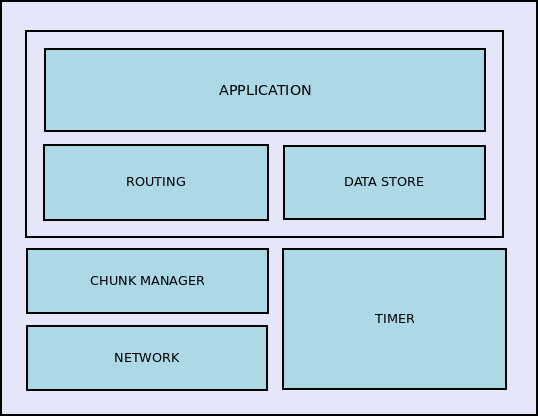
\includegraphics[width=8cm, height=12cm]{architecture_new}
	\centering
	\caption{Architectural Overview}
	\label{fig:architecture}
\end{figure}


%\begin{figure}[h]
%	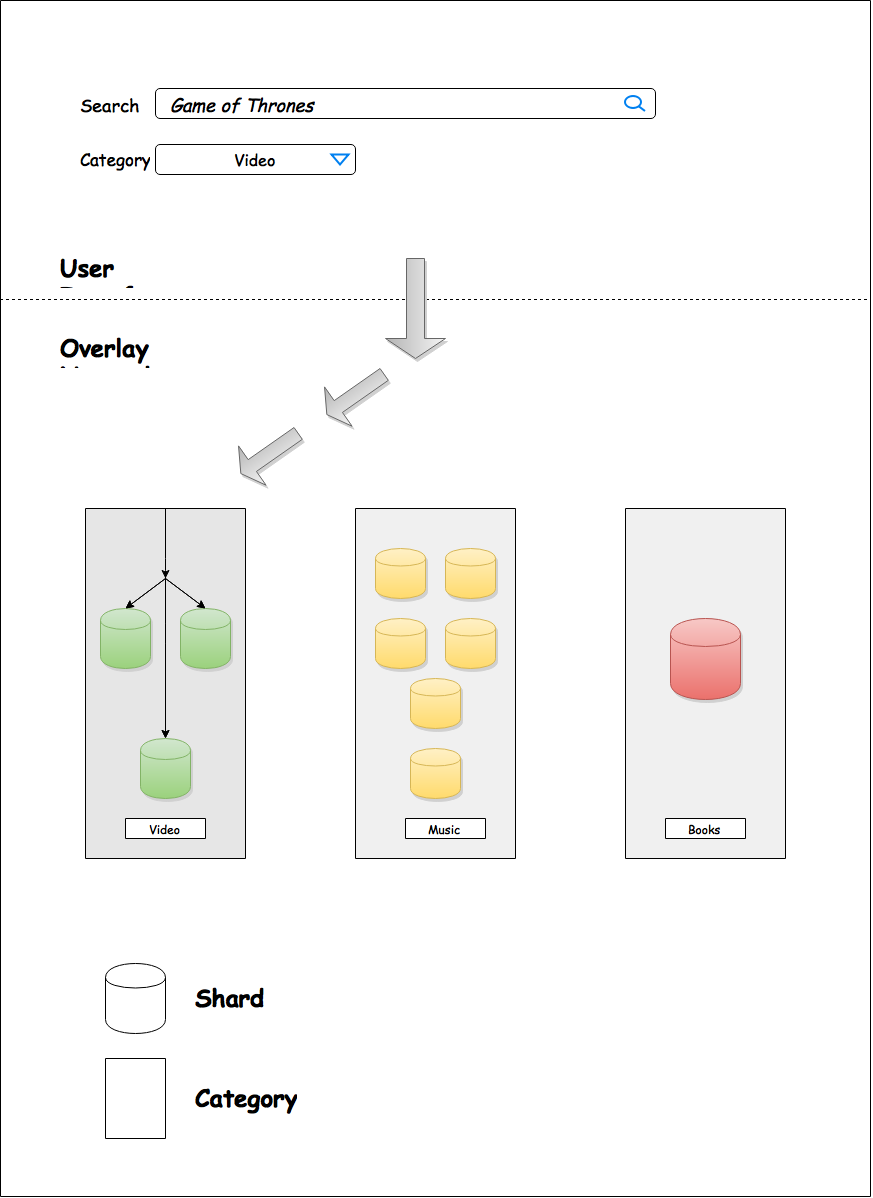
\includegraphics[width=10cm, height=12cm]{architecture}
%	\centering
%	\caption{Architectural Overview}
%	\label{fig:architecture1}
%\end{figure}

\subsection{Leader Election Protocol}
\label{ssec:leaderElection}

In context of distributed systems various leader election protocols have been discussed \cite{bully, lamportPaxos}. Election of leader for a group of nodes in the system typically requires all the nodes to agree upon the leader. Once the leader gets elected, it coordinates between the nodes and helps the group to move forward. 
\par As mentioned above, all the nodes usually need to know about the chapnode that would be elected as leader but in case of large scale system it would usually result in huge traffic in the system. As part of this thesis, we introduced a weaker form of leader election protocol known as \textit{Leader Selection}. As part of this protocol, we select a group of \textit{top K} nodes in the system. The node which has the highest utility among the K members tries to assert itself as the leader. Figure \ref{fig:p-arrange} provides a general overview of the system in which the top nodes are located at the center and as we go towards the edges of the system, the utility decreases as depicted by the color gradient. The node, in order to become the leader asks for promises from the other nodes in the selected group. In case, the nodes from the which the promises are sought, see anybody above the requesting node in terms of utility, rejects the promise. The requesting node which is trying to assert itself as leader, only moves to the commit phase after receiving promises from all the nodes in the group. In case any one of them rejects, the node resets the convergence counter and waits for the system to stabilize again. 

\par In order to better understand the mechanism, we need to look at the overlay over which the system is built. We use the Gradient topology, which is a class of P2P topology in which the nodes in the systems organize themselves in the network in such a way that the nodes with the highest utility  are concentrated at the center of the network and the nodes with low utility lies on the outer edges of the network. We use a \textit{preference function}, according to which nodes have a higher preference to form connections with the nodes which have utility higher but closer to itself. In this way the nodes arrange themselves in the system. The gradient sends sample of the preferred nodes to the application. The application on receiving the sample of preferred nodes, executes a convergence function in which it tries to calculate a percentage change in the number of neighbors. In case the change is greater than a predefined threshold \textit{D}, the node resets the convergence counter. On the other hand, if the change is below the threshold the node increments the counter. The node only tries to assert itself the leader, when the convergence counter has reached a certain value and the node based on its own utility sees no other node above it. It is only then, the node starts the promise round with the other K nodes. 

\par The main reason behind the use of convergence counter is due to the change in position of a node in the overlay. In case a node's utility decreases, its neighbors start forming connections with other nodes having higher utility and the node starts moving towards the edge of the system. Similarly, in case a node's utility increases, it starts moving up in the gradient during which it might be possible that during this rise, it doesn't locate any node above itself in terms of utility and wrongly thinks himself as leader. It could be avoided if the node looks at the change in the sample of neighbors provided by gradient on successive iterations and deduce that it is still rising in the gradient. Therefore, the main purpose behind convergence counter is to ensure that the position of the node has stabilized when it starts asserting itself as leader. 

\par This process of determining if self node is a leader is carried out by every node in every shard in the system. Eventually the leader gets elected for every shard. In addition to leader, every shard also has a follower group selected by the leader itself. The purpose of the follower group is to help the leader with the replication of the commands and the steps taken by the leader. In case the leader dies, the next higher node usually from the follower group takes over the leadership for that shard. The main functionality of the members of the followers group is as follows:


\begin{enumerate}

\item Reject all promises in case the node has already promised or is a part of follower group.

\item Accept a promise in case the node doesn't see anybody above the requesting node in terms of utility.

\item Expire a promise in case the commit message is not received before the timeout for a specific promise.

\end{enumerate}


As part of the leader selection mechanism, we try to elect a leader as soon as possible. In a very dynamic system where nodes can join and leave the system, it is very much possible that a better node comes along and try to assert itself as a leader even though a leader is already present thus violating the safety condition of having only a single leader per shard in the system. In order to prevent this, when a node gets elected as the leader, it along with the chosen follower group, artificially augments the utility by switching on the leader membership check. This check places the group at the center of the shard. In this way when a better node comes along, it cannot instantaneously start the election protocol because it's self membership check is switched off and it sees the current group as better than himself. 

\par It might be argued that the feature of artificially increasing the utility could lead to violation of fairness protocol, meaning that a node which became a leader initially, can become the leader for eternity in case the group membership check is not switched off. Therefore, it is the responsibility of the leader to locally switch off the leader group membership check and then look at the neighboring samples. In case the leader finds a better node, the leader simply backs of by terminating its membership. The follower group detects it and removes themselves from the group membership. The better node then starts the promise round itself and takes over the leadership for the current shard.

\begin{figure}[h]
	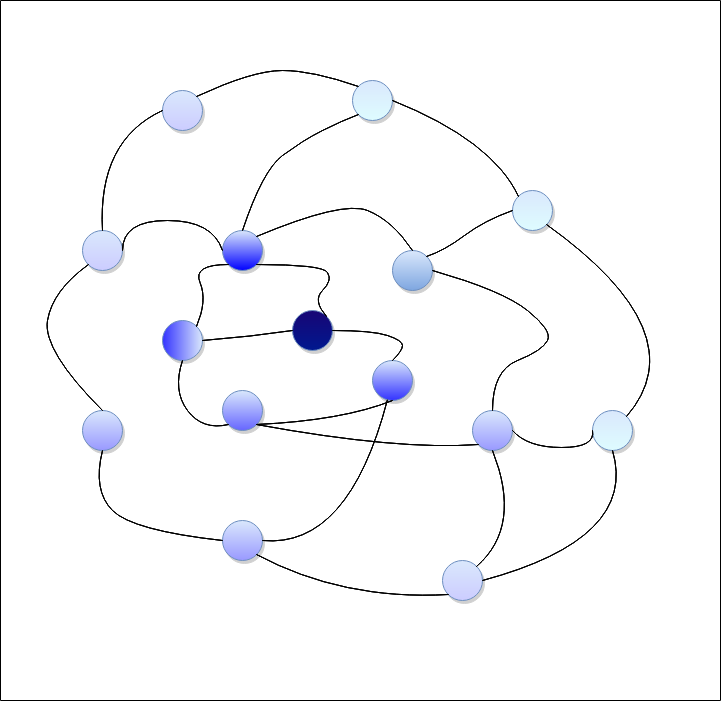
\includegraphics[scale=0.5]{p2p}
	\centering
	\caption{Peer Arrangement}
	\label{fig:p-arrange}
\end{figure}


\begin{algorithm}[h]
\caption{Eventual Leader Selection - Leader} 
\label{leader}
\begin{algorithmic}[1]
\Upon[init]{nodeId}
  \State $selfId := nodeId;$ $round := 0;$
  \State $isLeader := false;$ $stableGradient := false;$
  \State $gradSample := \emptyset;$ $followerGroup := \emptyset;$
  \TriggerS[periodicCheck]{}\EndTriggerS
 \EndUpon

\Upon[gradientSample]{sample}
  \State $stableGradient := $ \emph{stable}$(sample);$
  \State $gradientSample := sample;$
 \EndUpon

\UponS[periodicCheck]{}
  \If{$!isLeader$ AND $stableGradient$ AND \emph{highestUtility}$(selfId, gradientSample)$}
     \State $followerGroup := $ \emph{getTopK}$(gradientSample);$
     \ForEach[followerGroup]{member}
       \Trigger[promiseReq]{selfId, round} \EndTrigger
    \EndForEach
    \TriggerS[roundTimeout]{} \EndTriggerS
    \State $promiseSet := \emptyset$
  \EndIf
 \EndUponS

\Upon[promiseAck]{pNodeId, pRound}
  \If{pRound = round}
    \State $promiseSet := promiseSet \cup \{pNodeId\}$
    \If{followerGroup = promiseSet}
      \ForEach[followerGroup]{member}
        \Trigger[lease]{selfId}\EndTrigger 
      \EndForEach
      \State $isLeader := true;$
      \TriggerS[leaseTimeout]{}\EndTriggerS
      \TriggerS[cancelRoundTimeout]{}\EndTriggerS
    \EndIf
  \EndIf
\EndUpon

\Upon[promiseNack]{pNodeId, pRound} 
  \If{pRound = round}
    \State $round++;$
    \TriggerS[cancelRoundTimeout]{}\EndTriggerS
  \EndIf
\EndUpon

\UponS[roundTimeout]{}
  \State $round++$
\EndUponS

\UponS[leaseTimeout]{} 
  \State $sample := $ \emph{resetUtility}$(gradientSample);$
  \If{\emph{highestUtility}$(sample)$}
    \State $followerGroup := $ \emph{getTopK}$(sample)$
    \ForEach[followerGroup]{member}
      \Trigger[lease]{nodeId} \EndTrigger
    \EndForEach
    \TriggerS[leaseTimeout]{}\EndTriggerS
  \Else
    \State $isLeader := false;$
  \EndIf
\EndUponS

\end{algorithmic}
\end{algorithm}

\begin{algorithm}[h]
\caption{Eventual Leader Selection - Follower} 
\label{follower}Disadvantages
\begin{algorithmic}[1]

\UponS[init]{id}
  \State $isFolower := false;$
  \State $selfId := Id;$ $pendingPromise := Nil;$
  \State $gradientSample := \emptyset;$architecture
\EndUponS

\Upon[gradientSample]{sample}
  \State $gradientSample := sample;$
 \EndUpon

\Upon[promiseReq]{nodeId, round}
  \If{$!isFollower$ AND $pendingPromise = Nil$ AND \emph{highestUtility}$(nodeId, gradientSample)$}
    \State $pendingPromise := nodeId;$
    \Trigger[promiseAck]{selfId, round}\EndTrigger
    \TriggerS[promiseTimeout]{}\EndTriggerS
  \Else
     \Trigger[promiseNack]{selfId, round}\EndTrigger
  \EndIf
\EndUpon

\UponS[promiseTimeout]{}
  \State $pendingPromise := Nil;$
\EndUponS

\Upon[lease]{nodeId} 
  \If{$pendingPromise = nodeId $}
    \TriggerS[followerLeaseTimeout]{}\EndTriggerS
    \TriggerS[cancelPromiseTimeout]{}\EndTriggerS
    \State $isFollower := true;$
    \State \emph{setFollowerUtility}$();$
  \EndIf
\EndUpon

\UponS[promiseTimeout]{}
  \State $pendingPromise := Nil;$
\EndUponS

\UponS[leaseTimeout]{} 
  \State $isFollower := false;$
  \State \emph{resetFollowerUtility}$();$
\EndUponS

\end{algorithmic}
\end{algorithm}







\subsection{Preference and Utility Function}
\label{ssec:utility}
Each peer in the system has an associated utility based on the state of the peer at that instant. As the system evolves with time, so does its utility. As already mentioned, in order to build the overlay network, system uses a \textit {Preference Function} based on the utilities of the nodes. A peer uses this preference function mainly during the selection of peer for shuffling and to keep track of preferred neighbors. The preference function in case of the prototype developed is selection of the peers which have a higher utility than self but closer to self with higher probability. As seen in the Figure \ref{fig:preference}, if we assume utility having an absolute value, as per the preference function, \textit{Peer C} will prefer \textit{Peer A} over \textit{Peer B}, even though both have higher utility than C because A's utility is closer to utility of C.


\begin{figure}[h]
	\centering
	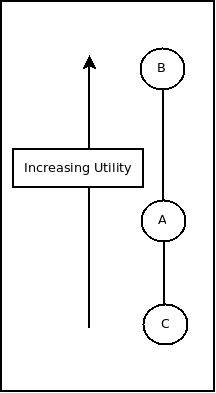
\includegraphics[scale=0.5]{preference}
	\caption{Utility Scale}
	\label{fig:preference}
\end{figure}




\par The preference function is based on the utility of a particular peer. It helps a peer to select a preferred peer from a collection of peers. The utility function is generally any metric or set of rules usually depending upon the application requirement which would help to create a total order on the peers in the system. In case of prototype developed as part of thesis, the utility function is as follows:

\small 
\begin{equation*}
    LeaderGroup \prec ReplicationScore \prec PeerScore \prec PeerID
\end{equation*}
\normalsize

While comparing the utility values of two different nodes, we simply compare them in the order defined above i.e from \textit {left to right}. We move on to the next parameter in the utility function in case total ordering cannot be achieved on the previous parameter. The utility comparison function starts by looking at the leader group membership check which indicates if a node is part of leader group for a particular shard. In case a node has this check switched on, the utility of the node suddenly increases compared to the other peers in the same shard. The Replication Score parameter indicates the number of the entries that a peer has its local lucene store. As system evolves and more entries are added in the shard the peer with a higher \textit{Replication Score} count indicates a better node in terms of serving latest entries added. Keeping in view the fairness protocol, we also have a \textit{PeerScore} metric in the utility function. This score helps to identify the peers with better resources in terms of computational capability, higher bandwidth. These nodes are given importance as they can easily serve a larger audience in the shard. The peer id is used a tie breaker in the function. We assume that the peers joining the system have unique identifiers.  In this way, we achieve a total order on the peers in the system.

\par The benefit of achieving total order on the nodes is the ability to assign ranks to the nodes with the lowest rank i.e. 0 being assigned to the \textit{leader} of the shard. As the system is continuously evolving, the utility of peers is changing and therefore the peers in the shard based on the neighboring peers can then adjust there own ranks. The purpose of assigning ranks is the creation of fingers which are nothing but long range links that each peer hold. Based on the rank, the peer usually try to find fingers i.e. links to the peers that are half its own rank. These fingers help speeding up the dissemination of the updates in the system.


\subsection{Pull Protocol}

The general overall functioning of the system involves electing a leader i.e a node with the highest utility as the leader of shard. The protocol employed for election of leader is \textit{Leader Selection} which is explained in detail in section \ref{ssec:leaderElection}. The leader is responsible for taking decisions regarding addition, searching of entries in the shard. In case of entry addition, in order to make the system highly available and prevent a single point of failure the leader performs a two phase commit to the nodes elected as part of leader group. Once the entry has been replicated to the leader group nodes, the leader returns back a successful response to the client. Now the peers can either push the entries to the neighboring nodes or nodes need to pull the entries added. The push protocol seems lucrative in terms that the peers as soon as they discover about a new entry, push the entry to other nodes. It prevents the other nodes constantly looking for the entries by asking the higher utility nodes. But there are major flaws in this scheme which are mentioned below:a high level view of the system involving routing requests to specific shards based on the category. In this section, we will be discussing its key modules.

\begin{enumerate}

\item From the security point of view, the push protocol is vulnerable to the Byzantine node attack. In case a node gets compromised, it can start pushing junk data to other nodes.


\item As the system is dynamic, nodes can arrive and leave the system at any time. A simple push protocol, prevents the node just joining the system to get all the updates pushed by the nodes higher in the utility prior to its joining.

\item A big flaw in using push protocol for the current prototype implementation is the way in which the preference function is defined. As mentioned earlier a particular node prefers node which higher but closer to itself in terms of utility. Therefore, given enough peers present above a particular node in terms of utility, that node will form all the neighborhood connections to the peers above itself. This tendency prevents nodes forming links with the peers on the edges of the shard i.e. the nodes having low utility. In absence of links, there is a high chance that the updates pushed by other nodes won't reach the nodes lower in the gradient.

\end{enumerate} 

As a result, we introduce pull protocol, in which the nodes constantly request the peers higher than self in terms of utility about any latest decisions taken in the shard by the leader. This way the information gets disseminated in the system. The dissemination protocol will be explained in greater detail in section \ref{ssec:gossip}



\subsection{Gossip Based Data Dissemination}
\label{ssec:gossip}
Once a node becomes a leader, it is implicitly trusted by other members in the shard. Initially the information of a node becoming a leader is only published at the leader group chosen by the leader. This information then gets pulled by other peers in the system. In this situation, it might be very much possible that a Byzantine Node might start publishing wrong information to the peers during the pull protocol. In order to avoid such situations, a peer during the pull protocol, requests updates from a predefined configurable peers usually three that are above itself in terms of utility.  The peers respond with the hashes of the information. Only the information for which the hashes match from all the nodes is then pulled from anyone of the responding peers. 
\par This approach is being used for securely disseminating the leader information in the system. In addition to this, entry dissemination is also based on this protocol. We think that this approach is secure enough in the sense that it is highly unlikely for all the nodes that are requested by peer to provide updates that are faulty.a high level view of the system involving routing requests to specific shards based on the category. In this section, we will be discussing its key modules.


\subsection{Load Balancing}
\label{ssec:loadBalance}
As the system evolves, the leader receives request for adding new entries in the system. Using basic replication strategies, the leader commits the entries to the leader group which then gets replicated to all the nodes in the shard using pull protocol. The system has a predefined \textit{MaxShardSize} parameter. When the entries grow beyond the count, the leader then initiates \textit{ShardSplit} protocol. As part of this protocol, each peer based on its identifier and its depth which is basically number of shard splits seen by the node, decides the next shard id. 
\par Before initiating the two phase commit of the shard split, the leader stops handling the entry additions. It then looks in its local lucene store and after sorting the entries based on their identifiers, calculates the split point. This meta information is then committed to the leader group nodes along with the shard split update as a part of two phase commit. Once the information is pulled by other peers in the system, based on there new shardId, they decide to remove all the entries either before or after the split point. The process of removing the entries in more detail when we introduce the concept of Leader Units and Timeline in section \ref{ssec:leaderUnit} and \ref{ssec:timeline} respectively. The peers then join the other peers in their respective shards. 



\subsection{Routing}
\label{ssec:routing}
utility
\par The client in order to look for the entries in the system generates a search request. The search request is then sent to the application running at the client node. The protocol of handling search request by the application involves locating the items matching the search request in the local data store. Once the matching items are located, necessary information is extracted from the items and response is generated to be sent back to the client. 

\par The above approach allows application to locate all the matching items in case all the data is located in the local data store. As part of load balancing protocol which explained in Section \ref{ssec:loadBalance}, the data gets distributed between the nodes in different shards. Now, it might be possible that the item that the client is looking for is located in other shards. Therefore, the application now needs to route the request to the nodes present in these shards. In order to do so, the application needs to have information about the shards and sample of nodes located in each shard. Therefore, each peer has a \textit{Routing} component which keeps track of the shards in the system and sample of nodes inside each shard. The component periodically gets random set of samples from the peer sampling service. Each node sample contains information regarding the shard to which it belongs to. Using this information, the component maps the descriptor to the shard. Now, when the application receives a search request, it gets information about all the shards and a set of descriptors in each shard. The query is then sent in parallel to all the shards. 


\subsection{Large Fanout}

In this section, we will be discussing the concept of \textit{latency variability} in large scale distributed systems. The term latency variability means the distribution of latency during an operation over the network. The importance of latency variability has increased in recent times due to the requirement for real time responsiveness of applications. Google quickly discovered that simply scaling the system doesn't necessarily means better performance during the response times of search requests \cite{tamingTail}. Normally the requests handled by a particular server are within the limits of respectable response times but once in a while the response time for a request would be much higher. This may be attributed to the network being slow due to choke or system disk from which the data is supposed to be read is acting slow. This phenomenon is known as long tail which has also been observed in trading systems where we might find the latencies of few trades in order of 900ms compared to normal latency of 5ms. 

\par We might argue that the occurrence of the phenomenon is not often enough to cause alarm but as the scale of the system keeps on growing as in case of Google where the data is divided into multiple shards, the search request needs to be fanned out to a larger audience and therefore the probability of occurrence of long tail increases as the requesting node needs to wait for responses from all the shards. This leads to unacceptable response times occurring with higher probability. 

\par Google uses a lot of innovative approaches to solve issue of latency variability as mentioned by Jeffery Dean in this talk \cite{jeffDean}. The approach that we are interested and have adapted for our prototype involves instead of sending to a single node in every shard the search request, we send it to a predefined number of nodes in that shard. We simply wait for the first response from that shard and discard the rest. The purpose behind it is to reduce the dependency on the slow performing node by replicating the request to other nodes within the same shard. Once all the shards have responded or search request timed out, we collect, filter and augment the results with some metadata. This data is then returned to the client. In this way the system makes significant steps towards preventing long tail in the search request's response times.


\chapter{Implementation}
\label{chap:impl}

In order to check for the viability of the theoretical approach we worked on developing a prototype on the principles stated in the design section. The prototype used Apache Lucene for storing and indexing data. In addition to this, the prototype was developed using the Kompics framework which is an asynchronous message passing system. The main application process on each node in the system is composed of following abstractions: \textit {group membership, routing, leader election} and \textit{data storage} abstraction. All the modules interact with the \textit{network} and \textit{timer} abstraction which are used to send messages over UDP and configure local timeouts respectively. In addition to this, we have a \textit{message chunking} abstraction which as name suggests check the messages going over the network and in case the message exceeds the maximum transmission limit, fragments the packet and at the receiving end joins the fragments to construct the final message. All of the abstractions are built from scratch in Java and have been previously explained in greater detail in Section \ref{sec:architecture}.

\par The application module as shown in Figure \ref{fig:architecture} is responsible for \textit{Indexing} and \textit{Searching} of the documents in the system. A high level view of the interaction of a single user layer with the system layer is shown in Figure \ref{fig:overall_function}. In case a node receives a request for adding an entry in the system, it forwards the request to the application module. The module firstly checks whether the node is the leader for the current shard. In case it is the leader, it invokes the entry addition routine on self. Otherwise, it sends the request to the routing module to route the request to the leader. As part of current implementation, the entry addition routine is a synchronous operation which involves performing a two phase commit by the leader over the leader group nodes. Only when the leader receives responses from the majority of leader group nodes, it commits the entry locally. In order to commit the entry the application module interacts with the data module to add the entry in the lucene. Once the entry gets replicated, the leader responds back to the node from which the request originated. 

\par The \textit{Search Entry Operation} involves user entering the name of the document to be located. The middle ware constructs a well defined search pattern which is understood by the lucene in the data storage abstraction. The search request is initially handled by the application module of the client. The application module sends this request to the routing module to check for the references of the nodes located in different shards in the system which are populated by the gossiping protocol constantly supplying random subset of the global samples to the routing module. The module then routes the request to multiple nodes in each shard. As the number of shards can grow therefore, it can easily result in large fanout search causing a long tail. To prevent this, we route request to more than one node in each shard and only handle the response from the fastest node and reject the other responses. The search responses are added in a separate lucene instance. In case all the shards responded or the timeout for search operation, whichever gets triggered first, the responses are then sorted and returned back to the client. 


\begin{figure}[h]
	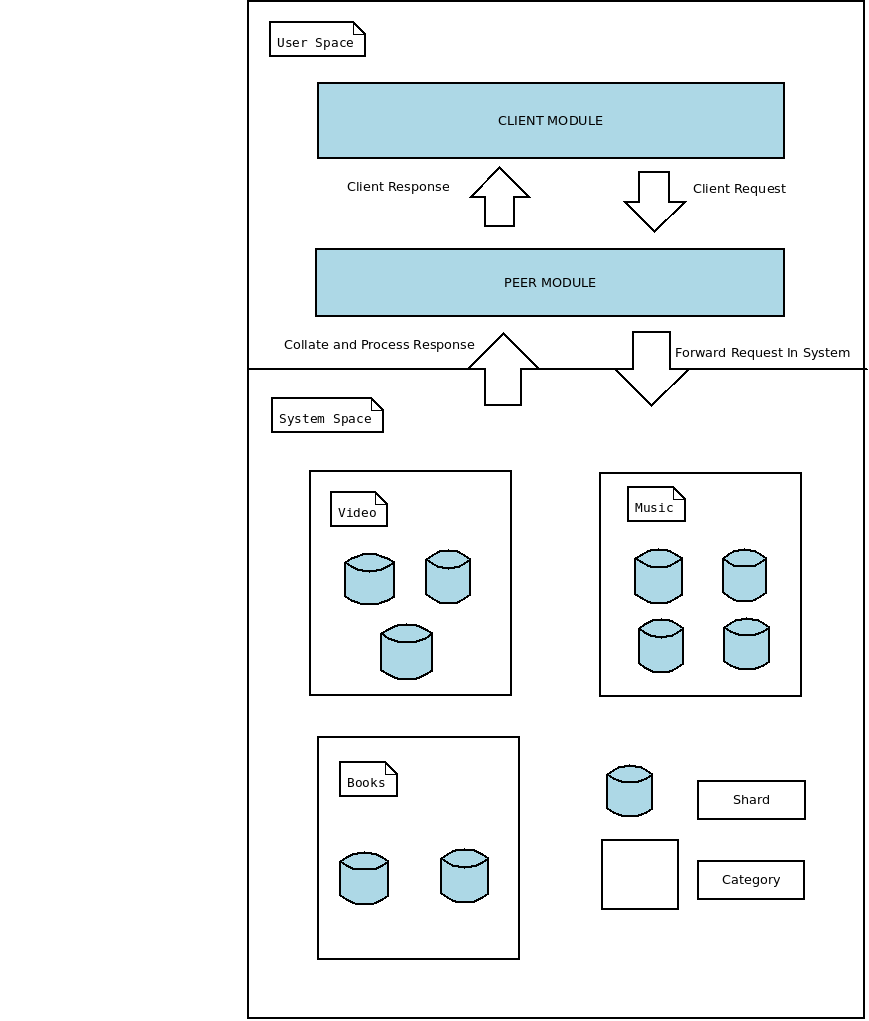
\includegraphics[scale=0.35]{OverallFunctioning}
	\centering
	\caption{Architectural Overview}
	\label{fig:overall_function}
\end{figure}



\subsection{Overlay Network}

The system strives to be a dynamic system in which the nodes can join and leave depending upon their requirement. Gradient topology built over peer sampling service is being used to construct the overlay of the system. The nodes perform shuffling as part of construction of a random graph and gradient topology over the random graph using preference function. Each node holds only a subset of total nodes which are known as preferred nodes. The mechanism to identify the preferred nodes depends upon the topology. The application holds two different set of preferred nodes, identified under the gradient and the peer sampling service. Each service keeps on updating the set by periodically identifying a node based on different policies and initiate a shuffle with that node. As part of shuffle nodes exchange a subset of the view held by them and merge in their local view the sample received from the other nodes. In this way, each peer is able to discover new peers joining the system. In addition to it, each sample also has an age attribute which gets incremented on every shuffle and helps to identify how long that particular sample has been in the system.

\par  As a node leaves the system voluntarily or by crashing, the sample of node in the system becomes stale. As an effort to keep neighborhood samples fresh, in case the size of the sample list grows beyond a predefined threshold, we removed the oldest sample i.e peer reference with the highest age. We quickly realized that if this approach needs to be successful, we would need to synchronize the rate at which the gradient and the peer sampling service performs shuffling with the neighborhood nodes.

\par In case the difference between the shuffling rates of both the services is large, the outcomes of the stabilization of the gradient were unexpected. The main reason behind it is that the peer sampling service feeds the sample to the gradient service. So in case the rate of shuffling in the sampling service is fast, the increment in the ages would be frequent because as part of shuffling the peers increment the age of the references and then exchange sample. Therefore the sampling service will feed the samples with high ages and the gradient shuffling is at a lower rate resulting in the slow rate of increase in ages. The nodes disseminate their updated utility in the system through the shuffles with age zero. Therefore, the node sample with a lower age would mean that it recently has been shuffled by the host node in the system and therefore indicates recent utility of the node. In case of difference in shuffling rates of the services with the sampling service shuffling faster than the gradient service, the probability of peer reference samples having ages higher than the corresponding samples present in the gradient sample is higher even though the peer reference from the sampling service has updated utility. Thus, the updated peer reference sample gets disseminated in the system slowly as the sample recent utility has a higher age than the same sample with old utility.

\subsection{Operations}
As part of current implementation, the prototype supports the following operations:

\begin{itemize}

\item \textit{add-entry (name, category, description, date)}
\item \textit{search-entry (name)}

\end{itemize}


\section{Entry Semantics}

\subsection{Entry Identifier Structure}
\label{ssec:entryIdStructure}
The structure of the identifier used by the system to identify the entries is mainly composed of three parts which will be briefly explained in this section:

\begin{tcolorbox}
\textbf{Identifier Structure:} \textless Epoch, LeaderId, EntryId \textgreater
\end{tcolorbox}

Whenever a client receives a request for entry to be added to the system, the request gets routed to the leader of the shard and the leader of the shard based on its own local state determines the identifier with which the entry will be added in the system. Therefore whenever a peer is chosen as a leader it will first identify different parts of the entry structure. 
\par Whenever a peer becomes the leader of the shard, it firstly identifies the epoch part of the entry structure. The \textit{Epoch} is simply a counter which is incremented by the node when it is chosen as leader. So whenever a peer is chosen as leader of the shard, it looks into its data store and identifies the epoch counter of the previous leader. In case if the node is the first leader in the system, the value of the epoch counter chosen is \textit{zero}, otherwise the peer increments the epoch of the previous leader by one. In addition to this, it also performs a commit over its leader group to inform them about the epoch with which it will be adding entries in the system. 
\par As part of current implementation, each leader will start adding entries under a particular epoch with the \textit{EntryId} part starting at \textit{zero} and being incremented on subsequent adds under same epoch. In addition to this, each node uses its own identifier which it gets at time of joining the system after booting up as the value for the \textit{LeaderId} part of the entry structure.  An invariant that we maintain is that each peer joins the system with a different identifier. Therefore at any given time in the system, there won't be any two nodes with the same  identifier. The reason behind the invariant is that the identifier of the node act as tie breaker in the preference function explained in detail in Section \ref{ssec:utility} and which is used to provide total ordering on the nodes. 

\par The main reason behind auto-increment of the entry id is to enable the nodes below in the system to identify the next entries to look for in the system. For example, if a node has already pulled an entry with entry id part of the entry structure as \textit{X}, it knows that the next entries for the particular epoch will be having entry identifier as \textit{X+1, X+2} and so on. Apart from this, the overall structure of the entry as a whole is chosen as to enable the creation of dense spaces. The requirement of dense space arise because of the issue of network partitioning. In a dynamic system which aims to run at hundreds of commodity machines, at any given time the nodes might be failing or the switches between the components might be broken. It can very well result in a network partition. As the system is self stabilizing, the nodes in the other partition will elect a new leader and evolve accordingly. When the partition heals and merge happens, we can now easily merge back the entries added in both the partitions because of these dense spaces. In order to better understand this, we can look at scenario in which there is a case of network partition and the each partition has elected its own leader. Let's say the identifier of two leaders are \textit{X and Y}. We also assume that both the leaders are operating in epoch \textit{E}. The entries added in this epoch are assigned entry identifier  incrementally starting from zero. Each leader starts committing the entries with a particular entry id which gets incremented on every subsequent entry add. Now when the network partition heals, we will have two sets of entries which can easily have the same epoch and the entry identifier value. In this case the presence of leader identifier in the entry structure ensures the uniqueness of each entry because the node which acted as leader can only be present in one of the partition. This scenario helps to establish the usefulness of the entry structure being used for the prototype. Figure \ref{fig:timelineMerge} presents the case of partition merge.

\par In above paragraph, we have identified the importance of the leader identifier and the entry identifier parts of the entry structure. The main use of the epoch identifier is help the system evolve with time. As new nodes gets elected as leader, they start adding entries with epoch identifier which is the increment of the epoch identifier of the previous leader. This process helps the system to identify the next entries to download once they have finished downloading the entries for a particular epoch. This nodes know that the next entries after the current epoch \textit{E}, if present will be with the epoch \textit{E+1}. Therefore, they start requesting the entries with the epoch \textit{E+1}. In this way, the nodes perform epoch switch and moves forward in the system.


\subsection{Leader Unit}
\label{ssec:leaderUnit}

A collection of entries added by a leader in a particular epoch is termed as a \textit{leader unit}. Each leader within a particular epoch can add only a specified amount of entries. As the number of entries reaches the threshold, the leader needs to perform a mandatory epoch switch. The structure of the leader unit is presented below:

\begin{tcolorbox}
\textbf{Leader Unit Structure:} \textless Epoch, LeaderId, NumEntries \textgreater
\end{tcolorbox}

The \textit{NumEntries} part of the structure identifies the number of entries added by a particular leader. The value of this parameter can be below the threshold in case the leader crashes before the unit is complete but it can never exceed the threshold. 

\par We limit the entries that a peer which is acting as a leader can add in order to balance the load on the newly created shards after sharding operation. As already explained in the section \ref{ssec:loadBalance}, during sharding phase, the leader calculates the split point identifier. It then performs a two phase commit over the leader group which gets pulled by other peers in the system. The split point is just used to identify the leader unit which will actually as a splitting point. We never remove the entries within the leader unit instead we keep or remove whole of the leader units. In order to keep things simple, each node based on predefined bitwise manipulation algorithm identifies whether the leader units less than the split point needs to be removed or split point leader unit and higher needs to be removed. The minimum load on the system before the leader initiates sharding protocol is \textit{ X * Max Leader Unit Entries} where X is a configurable number.



\subsection{Marker Entry}
Although the concept of peer informing the leader group about the current epoch on becoming the leader of particular shard has been introduced in previous sections, we will briefly explain the process in this section. 

\par Before a leader can start committing entries in a particular epoch, it needs to inform the other nodes in the shard about the epoch switch. The leader needs to make a \textit{marker entry} commit which will indicate the other nodes about the starting of the new epoch. The marker entry commit contains the maximum number of entries added by the previous leader. The current leader analyzes in its data storage module to calculate the entries added in the previous epoch. This information is committed to the leader group nodes which gets propagated to the system through the pull protocol.

\subsection{Timeline}
\label{ssec:timeline}
As the system is dynamic, any node can join and leave the system. In case the system has evolved enough and a new node joins the system, the new nodes also needs to pull entries from the neighboring nodes and evolve in the same manner to reach the stage at which the other nodes are present. Therefore the nodes in the system needs to keep track of the leader unit history. The timeline is an abstraction which mainly keeps track of the evolution of the system in terms of leader units added in the system.

\par At any moment in the system, the nodes in the leader group keep track of the latest updates to the shard in terms of entries being added or updated, leader unit switch happening because the previous leader crashed or maximum entries that a leader can add in the unit have been added and in order to continue the leader needs to perform a mandatory leader unit switch. All the other nodes needs to pull this information from the nodes higher in utility. In order to become aware of the next leader units each node request the nodes higher with the latest leader unit identified by the epoch, that it has seen. This information is stored in the timeline abstraction which is basically an In-Memory List as shown in Figure \ref{fig:timeline}. Each node to which the request is made looks locally in their timeline abstraction and returns the next in order leader units. Once the next leader units are verified by the requesting node, the application tries to add the leader units to the timeline. Under normal functioning, if the last leader unit in the timeline has epoch value \textit{X}, the next leader unit that the timeline will allow will be with value \textit{X+1}. The timeline buffers the unit updates which are not in order.

The information about the new leader units that are incorporated in the timeline is sent back to the application. This information is relayed to the entry pull protocol which needs to know about the next leader unit to pull from the higher nodes. In this way, the control pull protocol pulls and verify the next in order leader units and the entry pull protocol simply pulls the entries added in that particular unit. 

\par The leader units can contain maximum of \textit{N entries} or less which can happen because a leader can crash before completing the leader unit in which it was adding entries. Therefore the leader units added to the timeline can have different maximum entries. In case a node is allowed to pull out of order leader units, the leader unit will be picked up by the index pull protocol in the application. In case the number of entries in the unit are large, it can result in the node's utility being increased in higher proportion as compared to nodes which are pulling in order if the units they are pulling are having low maximum entries. This might result for the node to start its own voting protocol and  become a leader for the shard. In case the node succeeds, it will be having entry gaps concerning the absence of in order leader units. It won't be able to pull it from any other node as the node itself is the leader and doesn't have any higher utility node. Therefore, we maintain the invariant in which the timeline will not add and serve leader units out of order. 



\begin{figure}[H]
	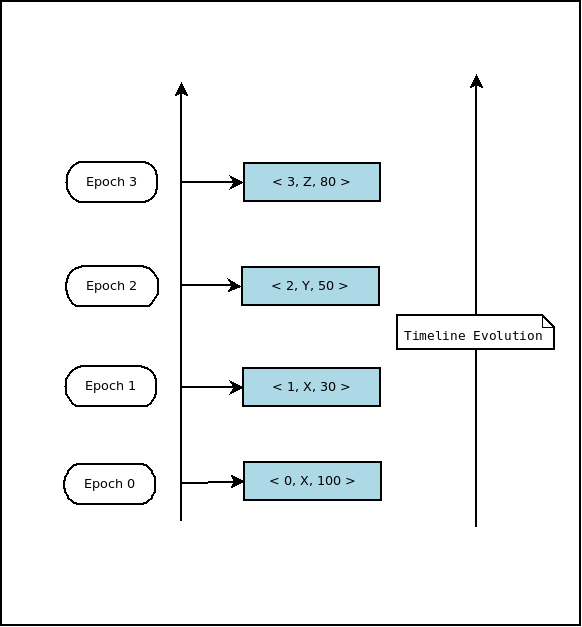
\includegraphics[scale=0.5]{timeline_new}
	\centering
	\caption{Timeline Evolution}
	\label{fig:timeline}
\end{figure}



\subsubsection{Skip Leader Units}

When a peer receives sharding update, the entry pull abstraction might currently be pulling a leader unit that is behind the sharding update or might have have already pulled all leader units before the sharding update. In any case, each peer gives priority to the sharding update. It pauses the current ongoing pull mechanism and analyzes the leader units that would have to be removed in case the node applies the update. Therefore, a node could realize that the leader units lying between e current unit that is being pulled and the sharding update are no longer required to be pulled as after applying the sharding update, these units would be removed.
\par The application needs to inform the entry pull protocol to skip some of the leader units. Therefore, each leader unit is provided with a status field which if set to \textit{SKIP} will be jumped over by the entry pull protocol. The application updates the timeline by updating the leader units that needs to be skipped by setting the status to \textit{SKIP}. Each peer has it's own set of leader units that needs to be skipped depending upon the units already pulled and units remaining between the last pulled and the sharding update. In best case scenario, the node could have pulled till the leader unit that will not be removed and the remaining ones needs to be Skipped. On the other hand, in worst case, a node could have already pulled all the leader units that would have to removed after sharding.

\subsubsection{Timeline Merge}
In section \ref{ssec:entryIdStructure} we introduced the concept of the dense identifier space created by the current identifier structure. In this section we will briefly explain the use of these dense spaces in event of network partition merge. 


\par As mentioned earlier, at any given moment in data center the router, network connection between the systems or the switches might be failing. It could easily result in an event of network partition in which a group of nodes might get separated and isolated from the other group. The system prototype is supposed to be highly available meaning that the system should function correctly in event of network partition. 

\par As it is not possible for the nodes to distinguish between the nodes getting partitioned or crashing, each group of nodes think that the nodes in the other group have crashed and they are ultimately removed from their view of system. The leader which was elected before the partition, keeps of functioning as the leader in one of the groups while the nodes in the other group realize about the death of their leader and start voting protocols to elect a new leader. Once a new leader gets elected, it choses its own leader group and informs about the epoch information with which it will be adding the entries. In this way, the two groups keep on evolving separately without knowing about the presence of other group which is depicted in Figure \ref{fig:timelineMerge}.

\par Usually, the network partitions are short lived. In case of network partition merge, usually through manual intervention, the nodes start discovering the other group of nodes. In order to merge the two partitions effectively the leader units that were added since the partition in both the branches needs to be identified and added to the leader group of the merged partition, which would be pulled by other nodes in the system. The dense spaces created by the entry identifier structure always allows entries added in two different branches to be identified uniquely. As we can see from the Figure \ref{fig:timelineMerge}, it is possible for the entries to be added in the two partitions with the same epoch and the entry identifier parts of the entry structure but the identifier of the leader that added the entries will be different because for a particular epoch, there could only be a single leader for a particular shard.

\par Once we identify the leader units that were added after the partition, they could easily be merged back in the timeline because of these dense spaces. Figure \ref{fig:timelineMerge} also depicts the above scenario of partition merge.



\begin{figure}[H]
	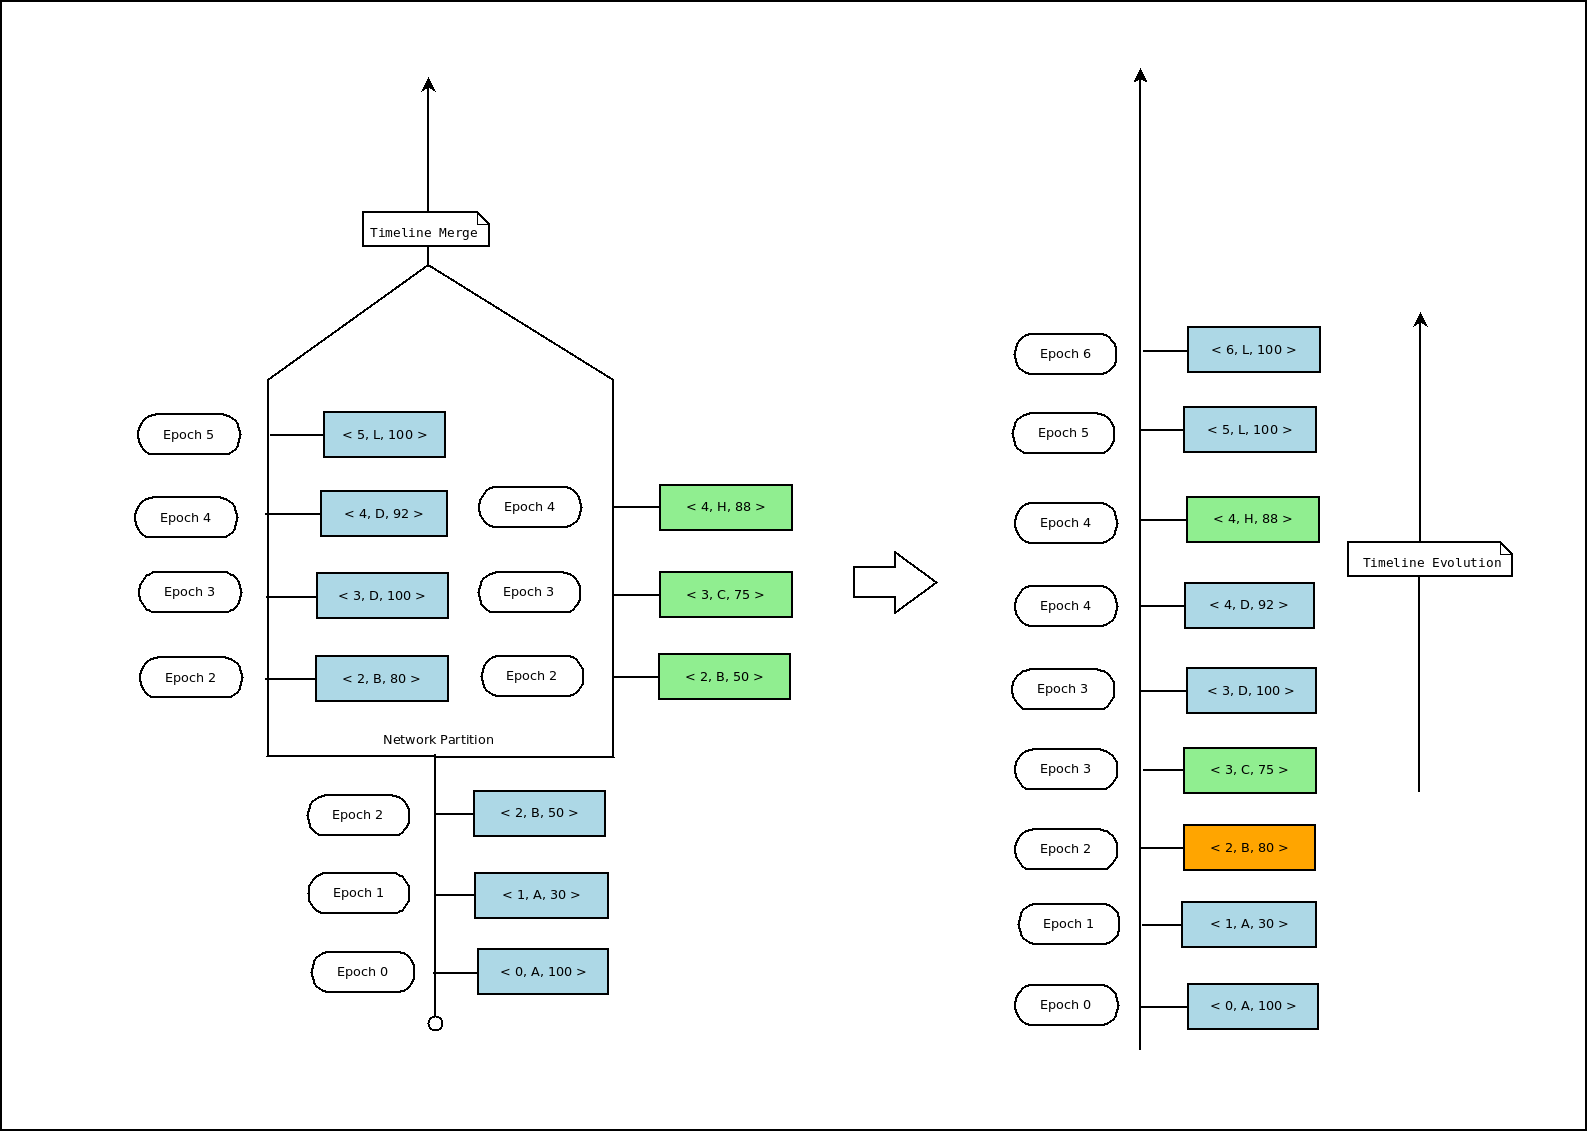
\includegraphics[width=14cm, height= 13cm]{timeline-merge}
	
	\caption{Timeline merge}
	\label{fig:timelineMerge}
\end{figure}


\newpage As we can clearly see from the Figure \ref{fig:timelineMerge}, a simple merge creates an issue of the split point leader unit. When the networks split, the nodes in one of the partitions assumed the current leader to be dead and started their own election protocols while the leader being alive in other partition continued with its operation. This can be seen from the differences in the leader units having the \textit{same epoch} and the \textit{leader identifier}  but different entries added in the system by the leader. When the partitions merge then the leader of the merged partitions need to identify the presence of this case and need to indicate the other nodes in the system to reopen the leader unit and fetch the remaining entries. The nodes which went into other partition than the leader at that time will recognize the difference in the entries and start pulling the remaining entries to become up to date.


\chapter{Evaluations}
\label{chap:eval}

In this section we will be discussing about the experiments that were performed as part of thesis to demonstrate the viability of the design.

\section{Experimental Setup}

The evaluations were performed on the machine with the following specifications:

\begin{itemize}
\item 8GB of RAM
\item Eight Cores (Intel(R) Core(TM) i7 CPU 860  @ 2.80GHz)
\end{itemize}

As mentioned earlier, the prototype is developed in Kompics which is an event driven asynchronous framework written in Java. Kompics has its own single threaded simulation environment. The nodes in simulation were booted up on a single machine as part of the experiment. In order to communicate with the nodes during different phases of the tests, a helper module was used to keep track of all the nodes started in simulation. A special node known as the \textbf{leader node} was also started with the lowest value of the identifier which allowed the node to become leader during the initial leader election phase. \\

Each peer in the system is composed of different components, each of which have there own well defined tasks. In addition to this, in order to track the overall health and status of the cluster, node responsible for aggregating information from all the nodes in the system is initiated. At fixed intervals, all components within a peer send their state to the a specialized local component known as \textbf{local aggregator} component. The component simply aggregates the data received and forwards it to the global aggregator component. In this way,  we are able to keep track of the overall status and health of the system.


\section{Workload Setup}

The simulations were executed on a cluster of two hundred nodes, unless otherwise explicitly stated. In order to assure the reproducibility of the results, the framework is inherently single threaded due to which the limiting factor concerning the scale of experiments was the strength of the processing unit of the machines used in simulation. \\

Below is the list of the different parameters that were tuned for the simulations:


\begin{itemize}
\setlength\itemsep{0em}
\item \textit{gradientViewSize} - 10 nodes
\item \textit{croupierViewSize} - 10 nodes
\item \textit{gradientShuffle} - 1000 (ms)
\item \textit{croupierShuffle} - 1000 (ms)
\item \textit{branchingFactor} - 10
\item \textit{electionConvergenceRounds} - 6
\item \textit{electionConvergenceTest} - 0.8d
\item \textit{Entry Pull Round} - 4000 (ms)
\item \textit{Control Pull Round} - 3000 (ms)
\item \textit{maxEntryExchange} - 25 nodes/ pull
\end{itemize}

In addition to the above parameters, an important parameter is the minimum number of nodes that a particular node needs to locate above itself in terms of utility, to pull the control or the entry information. As part of the experiments, the value of the parameter is set to three. This condition is respected by each node unless they find the leader in their local view in which case they directly pull the information from the leader thereby implicitly trusting the information provided by it.


\section{Convergence Experiment}

The \textit{Convergence Experiment} helps to understand the rapidness with which the entry gets disseminated in the system. As part of this experiment, we booted up 250 nodes in simulation. Once the system was stabilized in terms of leader of the shard getting elected and the marker entry for the current epoch being published by the leader and disseminated to each node in the system, we then added a single entry to the leader and analyzed the time it took for the entry to be disseminated to all the nodes in the system. The results as shown in Figure \ref{fig:250conv} points out that it took 8 - 9 (sec) for all the nodes to get the entry. This time evaluates to roughly two pull rounds based on the value of the current pull round timeout.

\begin{figure}[h]
	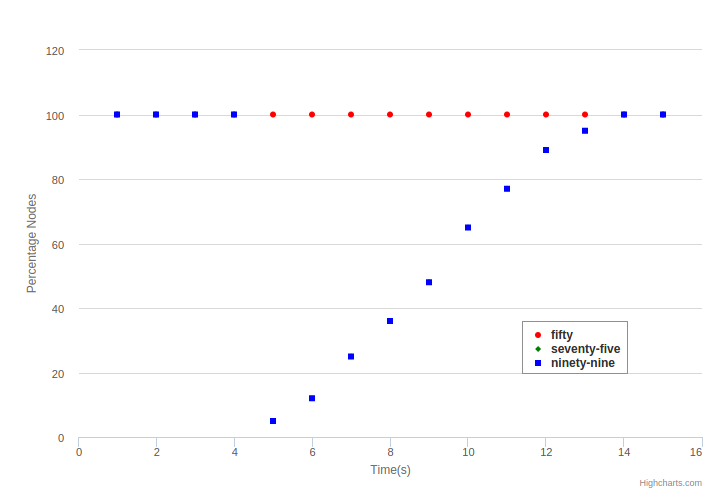
\includegraphics[scale=0.5]{250Convergence}
	\caption{Convergence - 250 nodes}
	\label{fig:250conv}
\end{figure}


Figure \ref{fig:500conv} shows the same experiment but now with 500 nodes in the simulation. The outcome is same as the previous one. The reason is because of the \textit{branchingFactor} parameter which is set to 10. Based on the parameters for the current simulation, the top 600 nodes in the system are expected to receive the information within two pull rounds. The results of the experiment conform with the expected outcome.


\begin{figure}[h]
	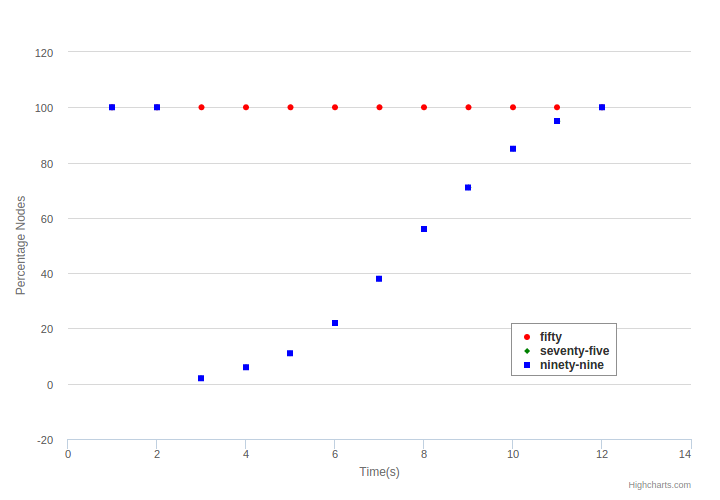
\includegraphics[scale=0.5]{500Convergence}
	\caption{Convergence - 500 nodes}
	\label{fig:500conv}
\end{figure}


\section{Add Entry Throughput}

In this experiment, we initially booted up 200 nodes in simulation. Once the gradient and the leader group became stabilized, initial batch of 20 entries were added in the system. We then started adding entries at varying rates likes \textit{1 entry per sec}, \textit{2 entries per sec} and  \textit{6 entries per sec} for a fixed period of time. As part of this experiment, we analyzed the fifty, seventy five and ninety nine percentile values i.e. number of nodes which at any given time during the operation of entry addition have fifty percent, seventy five percent and ninety nine percent of the total entries added in the system. 

\par The Figure \ref{fig:addEntry1} depicts the outcome in case of \textit{1 entry per sec}. As we can see the fifty percentile metrics seems stable as in all the nodes during the entry addition phase have atleast fifty percent or more of the entries. In case of seventy five percentile, it depicts a seesaw like structure. This behavior of the system initially looks strange but a closer look at the interaction of the application with the overlay over which the system is built can help to understand this behavior. As mentioned earlier, a node in order to perform a control pull needs to have atleast three nodes above himself in terms of utility. The node then matches the responses and incorporate the common in order responses in their local \textit{timeline}. As node mainly fetches the leader unit updates through the control pull, the entry pull mechanism takes this updated information about the number of entries in the system, requests for the next entries from the nodes above it. The mechanism of matching the responses is same as in case of control pull protocol. 

\begin{figure}[h]
	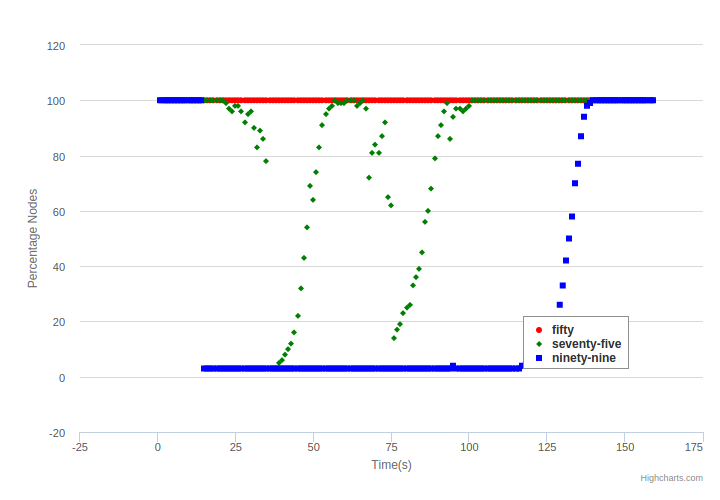
\includegraphics[scale=0.5]{200-1EntryPerSec}
	\caption{Add-Entry 1 entry(s)/Sec}
	\label{fig:addEntry1}
\end{figure}

\par The node then incorporates the entries by adding them to the Lucene Store and augmenting the utility accordingly. The application then informs the other components about its updated utility which allows them to make informed decisions. The overlay network contains a view of subset of total nodes in the system based on the preference function. With a sudden increase in the utility the local view of the gradient becomes obsolete and therefore the number higher samples return by the gradient to the application diminishes. In case a node unable to find desired number of higher utility nodes for the control pull simply it times out and wait for the next round to start. It is because of the obsolete view of the system in the gradient, the node doesn't initiate the control pull. In absence of the updated information about the entries in the system, the entry pull mechanism is unable to pull the next entries which are getting added to the leader and being replicated on the leader group nodes. Therefore the nodes in range of seventy percentile drops. Once the local view gets refreshed due to continuous shuffling and nodes injecting updated utilities in the system, the nodes are again able to find other nodes above themselves and start pulling the control information again resulting in the new entries being pulled.

\par Figure \ref{fig:addEntry6} depicts the performance of the system in event of addition of \textit{6 entries per sec}. The seesaw like structure can now be observed both in the fifty and seventy-five percentile. The reason being same as mentioned above. As the nodes near to the center of the gradient waits for the gradient to stabilize to get updated information, the nodes farther away near to the edges of the gradient are also unable to get the updated information. Therefore they also start lagging in terms of catching up to the leader group with has the latest information in terms of entries being added in the system. Apart from this, as observed from the diagrams the ninety percentile is really low in range of \textit{1-3\%}. The reason for this is because of the entries present in the system. As the entries that are added are usually low in addition to the initial entries, even a difference of one entry will remove a particular node from the ninety percentile. Therefore only the leader group nodes to which the leader replicates the entry being added are present in this range.

\begin{figure}[h]
	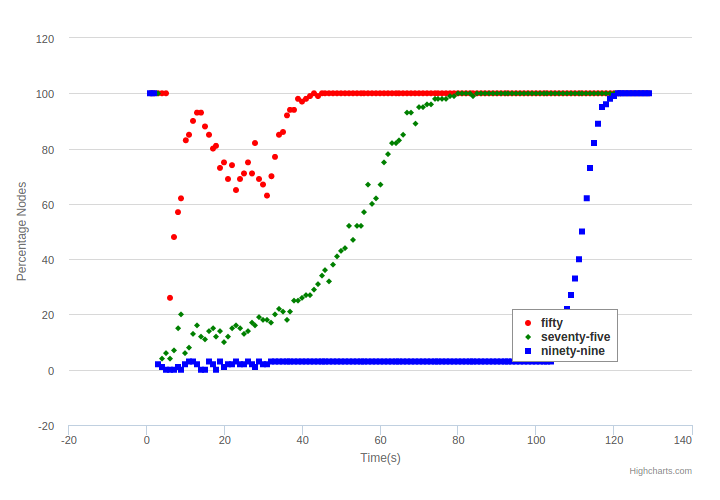
\includegraphics[scale=0.5]{200-6EntryPerSec}
	\caption{Add-Entry 6 entries/Sec}
	\label{fig:addEntry6}
\end{figure}

\section{Churn Experiment}

As part of this experiment, we initially started the system with 200 nodes and loaded the cluster with 100 entries. We started with the addition and the simultaneous removal \textit{4 Nodes per sec} to and from the system respectively. We continued this behavior for \textit{60 Seconds} thus resulting in a churn of \textit{four percent}. Nodes from the system except the nodes from the leader group were selected randomly to be removed by crashing and then stopping the nodes. New nodes were booted up with different node identifiers and added to the system. In addition to this, a constant rate of \textit{1 entry per sec} was employed for the entry addition. Figure \ref{fig:churn} depicts the fifty, seventy five and the ninety percentile values. As we can see more than fifty percent of the nodes had fifty and seventy percent of the entries at all times during the experiment. Only the leader group nodes seemed to be in the category of nodes having ninety nine percent of the entries at all times. 

\begin{figure}[h]
	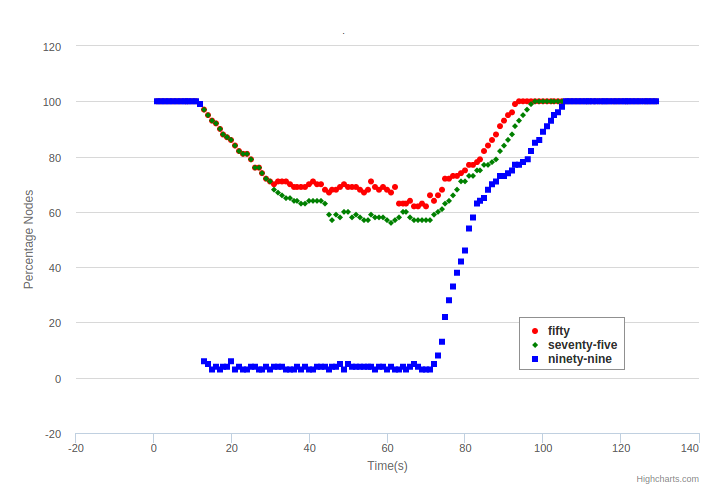
\includegraphics[scale=0.5]{200-4Node-1Entry}
	\caption{Churn 4 nodes/sec and 1 entry/sec}
	\label{fig:churn}
\end{figure}

\section{Flash Crowd Experiment}
As part of this experiment we started with 200 nodes in the system and loaded the system initially with 100 entries. We then introduced a bunch of fresh nodes in the system in quick succession and analyzed the time it took for the nodes to catch up to the nodes already present in the system in terms of the entries already added to them. We performed the experiment for flash crowd size of \textit{10 percent, 20 percent and 40 percent} of the original nodes in the system. As we can see from Figure \ref{fig:flash40} and \ref{fig:flash80}, it it took the nodes approximately \textit{ 15 - 20 seconds} for the nodes to catch up in terms of having fifty percent of the entries with the nodes already present. In addition to this, the time taken by nodes to catch up with the seventy five and ninety nine of the entries is approximately in the same range. 

\begin{figure}[h]
	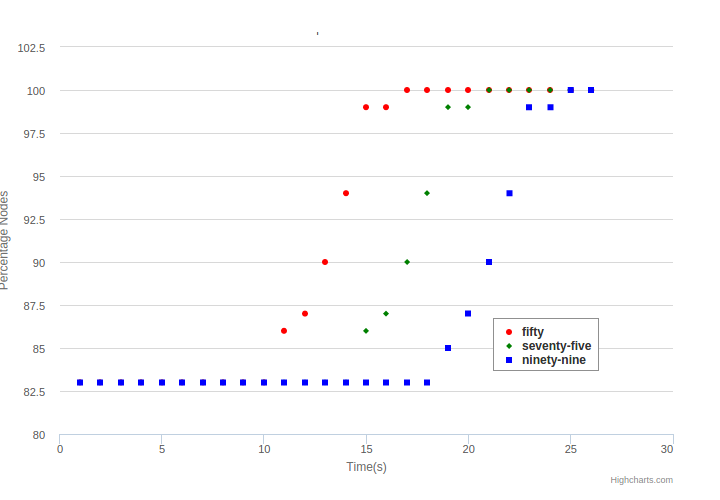
\includegraphics[scale=0.5]{200-40Nodes}
	\caption{FlashCrowd 40 nodes/Sec }
	\label{fig:flash40}
\end{figure}

\par Ideally as the \textit{maxEntryFetch} parameter per entry pull is \textit{twenty five}, it should take sixteen seconds i.e \textit{4 pull rounds} approximately for the nodes to fetch all the entries in the system but as observed from the diagram it takes more time than that. It is because it takes some time for the nodes to adjust themselves in the overall gradient and then pull the control information. Once the control information is pulled and verified, the nodes are able to determine the entries in the system at that moment and then start looking for the entries by requesting them from the nodes higher than themselves in terms of utility.

\begin{figure}[h]
	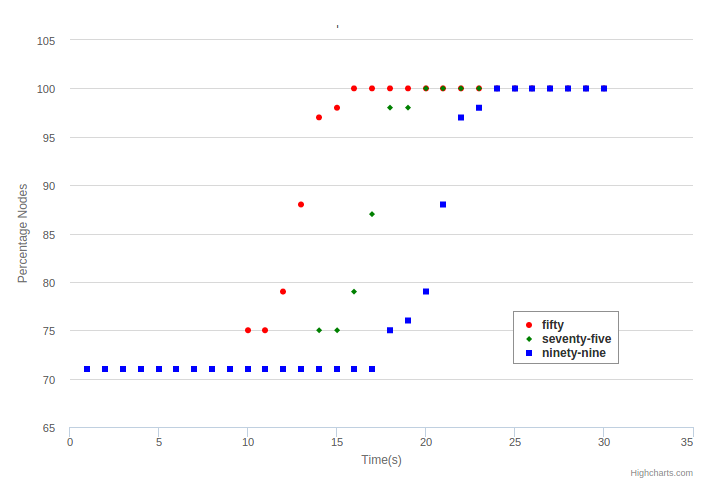
\includegraphics[scale=0.5]{200-80Nodes}
	\caption{FlashCrowd 80 nodes/Sec }
	\label{fig:flash80}
\end{figure}



\chapter{Conclusion}
\label{chap:conclusion}

As part of thesis, we introduced the architecture and design behind a Full Text Decentralized Peer to Peer Search System. In addition to this, we also developed a prototype based on the mentioned principles. The prototype is built over the overlay which in turn is constructed using gradient topology. The topology uses a preference function to form links with the preferred nodes in the system. As part of prototype, each node prefers nodes with higher utility but closer to them. In addition to this, in order to help with the coordination among the nodes, we introduced a weaker form of leader election protocol known as Leader Selection. Each node base on its local utility and neighbors determines its claim to become a leader for a particular shard and if the criteria is fulfilled initiates voting protocol. A peer once chosen leader for shard identifies the followers which are group of nodes over which the operations carries out by leader will be replicated. Leader also initiates a lease, after which it has to re-ascertain itself as a leader, failing which the follower group will remove it from the leader position and wait for another leader to emerge.
\par The whole system which is composed of a number of shards, is controlled by a small and fixed number of peers which are the leaders and its follower group for every shard. The prototype at present, exposes \textit{ADD} and \textit{SEARCH} entry operations. For adding a new entry, the request is redirected to the leader of shard which then replicates it over the follower group. Each node then pulls the information from the nodes above in the utility resulting in dissemination of the information in the system. In order to search, the request is sent to a random node in all the shards. The requesting node then wait for the responses from each shard after which it replies back to the client with relevant information. This fanout of search request to multiple shards is affected by latency variability wherein a single slow running node in one of the shards will affect the total response time of the shard request. To prevent this, the request is sent to multiple nodes in each shard and only response from the fastest node from each shard is considered.

\section{Future work}
\label{sec:future-work}
%% What you have left undone?
%% What are the next obvious things to be done?
%% What hints can you give to the next person who is going to followup upon your work?

The thesis presents a prototype implementation for the full text decentralized search based on Apache Lucene. The future work for the prototype built is briefly explained in below section:


\subsection{Delete and Update Operations}

As part of the implementation, the system only deals with the Add and Search entry operations. This greatly simplifies the execution as the entries are not modifiable and therefore the client needs to add a new entry with the updated values. In future, we would like to provide the user with update operation in which the application will still create a new entry to be added in the system but will delete the previous entry. The delete entry operation is difficult to implement because of the fact that the entry gets replicated to all the nodes in the system through the pull protocol. In order to implement a delete operation a special entry needs to be committed by the leader which would need to be pulled by the nodes in the shard and which will indicate delete operation for a particular entry from the datastore.

\subsection{Server Side Pagination}

Whenever a client initiates a search request, the number of matches for a particular search query could be very large. Sending all the data every time a search query is initiated can overwhelm the network. As part of current prototype implementation, to keep things simple we reply back with all the data matching the search query. In future as the amount of data in system will grow, this approach will become unfeasible. Therefore we would need to implement server side pagination, where in the client will generate the search request and send it to the server. The search request will also contain the page number and number of results which will enable the server to execute the query and sort the results and only return the results that would lie in that particular page number. If clients wont to see more responses, they will again initiate the same query but with a different page number to the server.


\subsection{Edge Case Identification}

As the system is asynchronous and composed of various components, each working independently of the other, certain edge cases exists for which the handling has not been defined. The priority will be to identify these cases and then handle them correctly. In addition to this, semantics of the fault handling and resolution is not defined yet. For now, in case of a fault like unable to write to data storage or individual components crashing, we simply throw an exception and crash the peer. This results in a poor user experience and therefore better fault handling and resolution needs to be carried out.


\subsection{Robust Sharding Protocol}
At present, the leader generates the splitting point and then each node based on the bitwise manipulation algorithm applied on its self identifier, decides to either remove the leader units above the splitting point or below it. This is a very basic approach. In future we would like to implement another bitwise manipulation algorithm which based on the metadata for each leader unit would identify the location of each leader unit after sharding. In this way the units could be transferred in different shards. The only drawback is that it would result in imbalance in load as it might be possible that the units identified to be sent to a particular shard have very less entries that the other ones meaning all the low capacity leader units might go in one shard and high capacity units in another shard. This problem needs to be solved before switching to the approach mentioned in this section.




\bibliography{report}
\bibliographystyle{IEEEtran}
%%\bibliographystyle{unsrturl}
%%\bibliographystyle{unsrtnat}
%%\bibliographystyle{myIEEEtran}
\appendix
%\chapter{Insensible Approximation}

%\backmatter

\end{document}
